\chapter{\selectlanguage{greek}Μέθοδοι προσομοίωσης}
Στο κεφάλαιο αυτό περιγράφεται η υλοποίηση του συστήματος, με βάση τη μελέτη που παρουσιάστηκε στο προηγούμενο κεφάλαιο. 
Αρχικά παρουσιάζεται η πλατφόρμα και τα προγραμματιστικά εργαλεία που χρησιμοποιήθηκαν. 

\section{Εργαλεία που χρησιμοποιήθηκαν}
Για την υλοποίηση των προσομοιώσεων χρησιμοποιήθηκε το πρόγραμμα \en{CST Particle Studio}, της σουίτας προγραμμάτων προσομοίωσης \en{CST Studio Suite}. 
Για την επεξεργασία των αποτελεσμάτων χρησιμοποιήθηκε το πρόγραμμα \en{MATLAB}. 
Τα προγράμματα παρουσιάζονται πιο αναλυτικά παρακάτω.

\subsection{Το \en{CST Particle Studio}}
\begin{figure}[tph]
\includegraphics[width=0.25\textwidth]{images/CST-logo.png}
\centering
\caption{Το λογότυπο του \en{CST}}
\label{img:CSTlogo}
\end{figure}
Το \en{CST PARTICLE STUDIO\textsuperscript{\textregistered} (CST\textsuperscript{\textregistered} PS) } είναι ένα εξειδικευμένο εργαλείο για την γρήγορη και ακριβή ανάλυση δυναμικών φορτισμένων σωματιδίων σε τρισδιάστατα ηλεκτρομαγνητικά πεδία.
Είναι ένα ισχυρό εργαλείο, κατάλληλο για μεγάλο φάσμα εργασιών, από σχεδιασμό \en{magnetrons} και ρύθμιση σωλήνων ηλεκτρονίως έως μοντελοποίηση πηγών σωματιδίων και εξαρτημάτων για επιταχυντές.

%\en{The particle tracking solver can model the behavior of particles through static fields, and with the gun iteration, space charge limited emission. 
Ο \en{particle-in-cell (PIC) solver}, ο οποίος μπορεί να λειτουργήσει στο πεδίο του χρόνου, μπορεί να εκτελέσει μια πλήρη προσομοίωση σωματιδίων και ηλεκτρομαγνητικών πεδίων.

Για σχετικιστικές εφαρμογής, ο \en{wakefield solver} μπορεί να υπολογίσει πώς τα πεδία που δημιουργούνται από σωματίδια που κινούνται στην (ή κοντά στην) ταχύτητα του φωτός, αλληλεπιδρούν με τη δομή γύρω τους.

Το \en{CST PS} έχει ενσωματωμένα τα \en{3D EM modules} του \en{CST STUDIO SUITE\textsuperscript{\textregistered}}, όπως τα \en{CST EM STUDIO\textsuperscript{\textregistered} electro- and magnetostatic solvers} και το \en{CST MICROWAVE STUDIO\textsuperscript{\textregistered} eigenmode solver}.

Είναι πλήρως ενσωματωμένα στο περιβάλλον σχεδίασης \en{CST STUDIO SUITE}, χρησιμοποιώντας έτσι τις δυνατότητες μοντελοποίησης και τα \en{import interfaces}.

Το \en{CST PS} βασίζεται στη γνώση, την έρευνα και την ανάπτυξη των αλγορίθμων που χρησιμοποιήθηκαν στο πακέτο προσομοίωσης \en{MAFIA-4}. 
Ο \en{PIC solver} μπορεί επίσης να εκμεταλλευτεί δυνατότητες \en{GPU computing}, προσφέροντας σημαντικές βελτιώσεις στην απόδοση, σε συμβατό υλικό.

\subsection{Το \en{MATLAB}}
Το \en{MATLAB (matrix laboratory)} είναι ένα περιβάλλον αριθμητικής υπολογιστικής και μια προγραμματιστική γλώσσα τέταρτης γενιάς. 
\en{A proprietary programming language developed by MathWorks, MATLAB allows matrix manipulations, plotting of functions and data, implementation of algorithms, creation of user interfaces, and interfacing with programs written in other languages, including C, C++, C\# , Java, Fortran and Python.}

\en{Although MATLAB is intended primarily for numerical computing, an optional toolbox uses the MuPAD symbolic engine, allowing access to symbolic computing abilities. 
An additional package, Simulink, adds graphical multi-domain simulation and model-based design for dynamic and embedded systems.}

\begin{figure}[tph]
\includegraphics[width=0.25\textwidth]{images/Matlab-logo.png}
\centering
\caption{Το λογότυπο του \en{MATLAB}}
\label{img:MATLABlogo}
\end{figure}

\section{Επιρροή διάφορων μεταβλητών σε έναν \en{Electron Beam Scanner}}
Όπως περιγράφεται και από \cite{Logatchov1999}, 

\en{The thin probe beam moves along $X$ axis, is orthogonal to the direction of the relativistic bunch motion ($Z$ axis) with the offset parameter} $\rho$ (Σχήμα \ref{fig:ellipse-EBS}).
\begin{figure}[tph]
\includegraphics{figures/Logatchov1999-EBS}
\centering
\caption{Διαδικασία ανίχνευσης της έλλειψης που χαρακτηρίζει τη δέσμη}
\label{fig:ellipse-EBS}
\end{figure}

\en{The results of scanning are monitored on the screen parallel to the $Y-Z$ plane and positioned at the distance $L$ from $Z$ axis. 
Let the center of the relativistic bunch is located at the origin at time $t=0$ whereas the testing beam has the uniform density along $X$ and the diameter $d \ll \rho$. 
Here, we assume $\rho$ exceeds the typical
transverse size of the relativistic bunch. 
At the time $t=0$ every testing beam particle is corresponded to the certain $x$-coordinate. 
The total deflecting angle in $Y$ direction for every particle under the influence of the electric field of the relativistic bunch can be expressed as:}
		\begin{equation}
			\theta_y (x) = \frac{2 \rho r_e}{\beta} \int_{-\infty}^{\infty}\frac{n(z) \dd z}{\rho^2 + \left(x+\beta z \right) ^2}
		\end{equation}
\en{where $r_e$ is the classical electron radius, $\beta =v_t/c$ - the relative velocity of the testing beam, $c$ - the velocity of light, $x$ - the coordinate of testing beam particle at $t=0$, $n(z)$ - the relativistic bunch linear density along $Z$ axis. 
The expression for the deflecting angle of the particle in $Z$ direction due to magnetic field can be written as:}
		
		\begin{equation}
			\theta_z(x) = 2 r_e \int_{-\infty}^{\infty}\frac{(x+\beta z)n(z) \dd z}{\rho^2 + \left(x+\beta z \right) ^2}
		\end{equation}
		Αυτά τα κάνουμε \en{plot} και είδαμε πώς επηρεάζονται από 
		\begin{itemize}
			\item \en{bunch intensity}
			\item \en{bunch length}
			\item \en{Y-offset} ($\rho$) 
			\item \en{probe beam voltage} 
		\end{itemize}   

\begin{figure}[tbh]
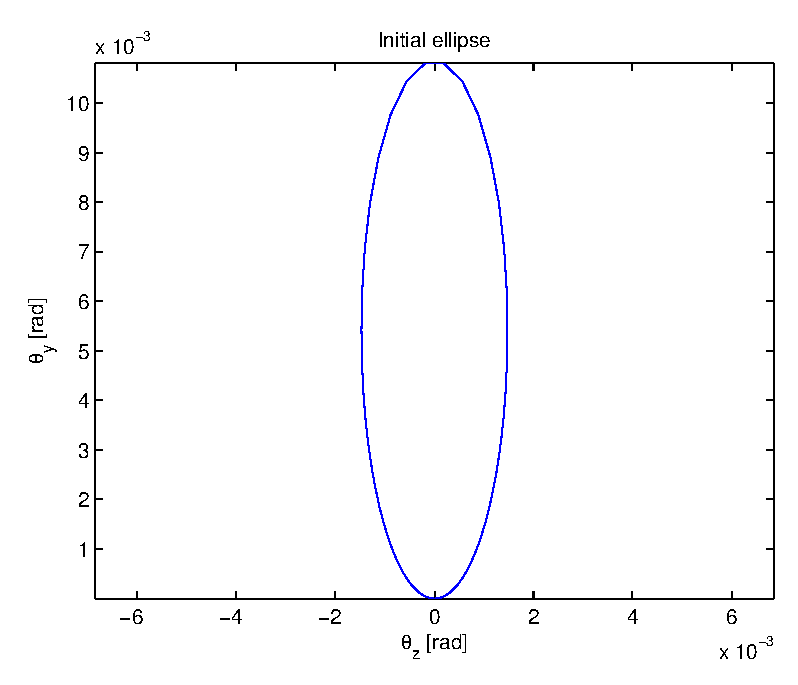
\includegraphics[width=0.75\textwidth]{figures/beam_deflection_script_01_initial_elipse}
\centering
\caption{Έλλειψη στην αρχική κατάσταση}
\label{fig:beam_deflection_script_01_initial_elipse}
\end{figure}

\begin{figure}[tbh]
\includegraphics[width=0.75\textwidth]{figures/beam_deflection_script_02_elipse_width}
\centering
\caption{Το πλάτος και ύψος της έλλειψης στην αρχική κατάσταση}
\label{fig:beam_deflection_script_02_elipse_width}
\end{figure}

\begin{figure}[tbh]
\includegraphics[width=0.75\textwidth]{figures/beam_deflection_script_03_elipse_height}
\centering
\caption{Επιρροή της έντασης της δέσμης στην ύψος και το λόγο της έλλειψης}
\label{fig:beam_deflection_script_03_elipse_height}
\end{figure}

\begin{figure}[tbh]
\includegraphics[width=0.75\textwidth]{figures/beam_deflection_script_04_elipse_height_by_bunch_intensity}
\centering
\caption{Επιρροή του μήκους της δέσμης στην ύψος και το λόγο της έλλειψης}
\label{fig:beam_deflection_script_04_elipse_height_by_bunch_intensity}
\end{figure}

\begin{figure}[tbh]
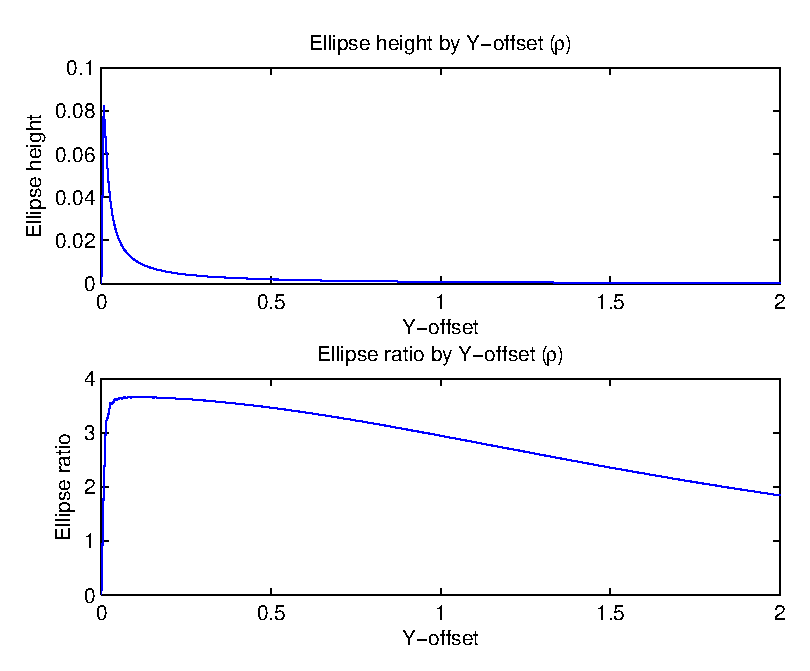
\includegraphics[width=0.75\textwidth]{figures/beam_deflection_script_05_elipse_ratio_by_bunch_intensity}
\centering
\caption{Επιρροή της αρχικής θέσης ριπής ($Y$-\en{offset} της δέσμης στην ύψος και το λόγο της έλλειψης}
\label{fig:beam_deflection_script_05_elipse_ratio_by_bunch_intensity}
\end{figure}

\begin{figure}[tbh]
\includegraphics[width=0.75\textwidth]{figures/beam_deflection_script_06}
\centering
\caption{Επιρροή της γραμμικής μεταβολής τάσης της δέσμης στην ύψος και το λόγο της έλλειψης}
\label{fig:beam_deflection_script_06}
\end{figure}

\begin{figure}[tbh]
\includegraphics[width=0.75\textwidth]{figures/beam_deflection_script_07}
\centering
\caption{Επιρροή της εκθετικής μεταβολής τάσης της δέσμης στην ύψος και το λόγο της έλλειψης}
\label{fig:beam_deflection_script_07}
\end{figure}

\section{Ανάλυση με το \en{CST Particle Studio}}

\begin{figure}[tbh]
\includegraphics[width=0.5\textwidth]{figures/CST-main-beam-source}
\centering
\caption{Η πηγή της δέσμης στο \en{CST}}
\label{fig:CST-mainBeamSource}
\end{figure}

\begin{figure}[tbh]
\includegraphics[width=\textwidth]{figures/CST-pic-monitor}
\centering
\caption{Η διάταξη προσομοιωμένη στο \en{CST}}
\label{fig:CST-PICmonitor}
\end{figure}
